\documentclass[times, utf8, zavrsni, numeric]{fer}
\usepackage{booktabs}
\usepackage{float}
\usepackage{braket}
\usepackage{tikz}
\usepackage{quantikz}

%\ignorecitefornumbering
% za kod
\usepackage{listings}
\usepackage{xcolor}
\definecolor{codegreen}{rgb}{0,0.6,0}
\definecolor{codegray}{rgb}{0.5,0.5,0.5}
\definecolor{codepurple}{rgb}{0.58,0,0.82}
\definecolor{codeblue}{rgb}{0.23,0.22,0.97} % 60, 57, 247
\definecolor{backcolour}{rgb}{0.95,0.95,0.95}
\lstdefinestyle{mystyle}{
    backgroundcolor=\color{backcolour},   
    commentstyle=\color{codegreen},
    keywordstyle=\color{codeblue},
    numberstyle=\tiny\color{codegray},
    stringstyle=\color{codepurple},
    basicstyle=\ttfamily\footnotesize,
    breakatwhitespace=false,         
    breaklines=true,                 
    captionpos=b,                    
    keepspaces=true,                 
    numbers=left,                    
    numbersep=5pt,                  
    showspaces=false,                
    showstringspaces=false,
    showtabs=false,                  
    tabsize=2
}



\begin{document}

% TODO: Navedite broj rada.
\thesisnumber{228}

% TODO: Navedite naslov rada.
\title{Simulacija kvantnog računala}

% TODO: Navedite vaše ime i prezime.
\author{Dominik Matić}

\maketitle

% Ispis stranice s napomenom o umetanju izvornika rada. Uklonite naredbu \izvornik ako želite izbaciti tu stranicu.
%\izvornik

% Dodavanje zahvale ili prazne stranice. Ako ne želite dodati zahvalu, naredbu ostavite radi prazne stranice.
\zahvala{}

\tableofcontents
 
%\chapter{Uvod}
%Uvod rada. Nakon uvoda dolaze poglavlja u kojima se obrađuje tema.

\chapter{Uvod}
\label{ch:uvod}
Neprestanim razvojem znanosti i tehnologije, kvantna računala postaju sve bitnijim dijelom računarstva. Predstavljaju sasvim drugačiji način računanja koji otvara vrata rješavanju mnogih problema koje klasično računalo, zbog same prirode problema, ili rješava znatno sporije ili uopće ne može riješiti u razumnom vremenu. Takvi problemi javljaju se u područjima kriptografije, umjetne inteligencije i strojnog učenja, računalne biologije, financija, simulacije kvantnih sustava kao i u ostalim područjima računarstva kao što su algoritmi pretraživanja.

Područje kriptografije je posebno zanimljivo jer se većina današnjih sigurnosnih mehanizama interneta temelji na matematičkim problemima za koje se smatra da su teško izračunljivi. To su primarno problem faktorizacije velikih brojeva te problem diskretnog logaritma. Kvantno računalo efikasno rješava takve probleme, što je još devedesetih godina demonstrirao Peter Shor\citep{Shor:1994jg}. Naravno, iz toga slijedi da će kvantna računala biti velika prijetnja sigurnosti na internetu, no već su se počeli razvijati mehanizmi koji će biti otporni na napade kvantnim računalom[citati?] što  samo govori o tome koliko je kvantno računalo blizu da postane veliki dio računarstva.

Potencijal kvantnog računala poznat je desetljećima te su već smišljeni i detaljno opisani mnogi od algoritama prikladni za takav način računanja. Sve što je preostalo je izgraditi računalo koja će moći provoditi te algoritme. Danas, IBM posjeduje kvantno računalo s najvećim brojem kvantnih bitova, njih čak 65, no ni to još nije dovoljno da bude korisno. Naime, problem nastaje s pojavom kvantne dekoherencije. Dekoherencija predstavlja gubitak informacije kvantog sustava zbog interakcije s okolinom što onemogućava precizno ili čak bilo kakvo računanje. No, kvantno računarstvo je trenutno veliki predmet istraživanja te se napretci ostvaruju skoro svaki dan. Mogućnost izgradnje kvantnog računala sa dovoljno velikim brojem kvantnih bitova je sve izglednija, kao primjer, IBM obećava do 2023. godine izgraditi kvantno računalo sa 1000 kvantnih bitova\citep{ibm:quantum}.

S ciljem demonstracije nekih od mogućnosti kvantnog računala, ovaj rad se u provm dijelu bavi osnovnim načelima kvantnog računala, tj. matematičkim modelom kojim opisujemo kvantnomehaničke pojave koje nam omogućuju drugačiji način računanja. Nakon toga rad opisuje neke od algoritama namijenjenih za kvantno računalo te ćemo zatim neke od njih implementirati i demonstrirati u samostalno izgrađenom simulatoru.

\chapter{Kvantno računalo}

\section{Polarizacija svjetlosti}

Klasična fizika shvaća svjetlost kao transverzalni elektromagnetski val koji može biti poraliziran na različite načine. Polarizacija svjetlosti određena je njenom električnom komponentom te je svjetlost koju emitiraju prirodni izvori svjetlosti uglavnom nepolarizirana. Tek kada se snop svjetlosti pusti kroz polarizator dobije se linearno polariziran val svjetlosti --- val koji ima stalni smjer širenja okomit na smjer titranja. Njegova električna komponenta dana je jednadžbom:
\begin{equation}
E = E_0 \hat{p}e^{i\omega t}
\end{equation}
gdje je $\hat{p}$ jedinični vektor u smjeru polarizacije vala. Intenzitet ovako polariziranog vala biti će upola manji od intenziteta početnog nepolariziranog vala jer će točno toliko intenziteta polarizator apsorbirati. Kada ovakav val pustimo kroz još jedan polarizator (tzv. analizator), val koji ćemo dobiti jest:
\begin{equation}
E' = (E \cdot \hat{n}) \hat{n} = E_0 (\hat{p} \cdot \hat{n})\hat{n}e^{i\omega t} = E_0 \cos \alpha
\end{equation}
gdje je $\hat{n}$ jedinični vektor u smjeru polarizacije analizatora, a $\alpha$ kut između vektora $\hat{p}$ i $\hat{n}$. Intenzitet novog vala dobivamo po Malusovom zakonu:
\begin{equation}
I' = I \cos^2 \alpha
\end{equation}
gdje je $I$ intenzitet prethodno polariziranog vala. Drugim riječima, polarizacijom vala dobivamo njegovu projekciju na ravninu određenu kutom polarizatora. 

U kvantnoj mehanici, svjetlost je definirana drugačije --- kao niz fotona, nedjeljivih elementarnih čestica. Kod takve interpretacije postavlja se pitanje što se događa kada individualni fotoni prolaze kroz polarizator. Ako polarizator propušta projekciju, koja je uvijek manja ili jednaka ulaznom valu, što će se dogoditi fotonu, ako je on nedjeljiv? Eksperimenti su pokazali da će foton sa točno određenom šansom ili cijeli proći kroz polarizator sa novim smjerom polarizacije ili biti apsorbiran. Ključan element takvih eksperimenata je činjenica da je nemoguće \emph{niti u načelu} odrediti što će se dogoditi sa fotonom. To znači da čak uz poznavanje svih varijabli nekog sustava, nemoguće je deterministički odrediti ishod.

Prijelaze kvantnih sustava iz jednog stanja u drugo modeliramo takozvanom amplitudom vjerojatnosti:
\begin{equation}
a(\phi \rightarrow \psi)
\end{equation}
koja je element skupa kompleksnih brojeva, a vjerojatnost da neki sustav koji je u stanju $\phi$ bude izmjeren u stanju $\psi$ dobivamo na način:
\begin{equation}
p(\phi \rightarrow \psi) = |a(\phi \rightarrow \psi)|^2
\end{equation}

U slučaju polarizatora, vjerojatnost smo mogli izračunati pomoću Malusovog zakona što nam daje vjerojatnost prolaska fotona kroz polarizator jednaku
\begin{equation}
p(\phi \rightarrow \psi) = \cos^2 \alpha
\end{equation}
iz čega je vidljiva amplituda vjerojatnosti:
\begin{equation}
|a(\phi \rightarrow \psi)|^2 = \cos^2 \alpha \Rightarrow a(\phi \rightarrow \psi) = \cos \alpha
\end{equation}
gdje je $\alpha$ kut koji zatvaraju vektori polarizacije fotona i polarizatora, $\phi$ stanje fotona prije prolaska kroz polarizator, a $\psi$ stanje u kojemu foton nije apsorbiran.

%Sličan primjer polarizatoru je dvolomac koji također funkcionira kao polarizator, samo što ne apsorbira svjetlost, nego dijeli svjetlost na dva ortogonalno polarizirana snopa. Koristeći dvolomac moguće je pomoću dva detektora izmjeriti u kojem je točno stanju foton završio. Nakon mjerenja, tj. detekcije, foton je apsorbiran.


\section{Kvantni bit}

\subsection{Svojstva}
Umjesto polarizatora moguće je koristiti i dvolomac koji također funkcionira kao polarizator, samo što ne apsorbira dio svjetlosti, nego dijeli svjetlost na dva ortagonalno polarizirana snopa. Kombinirajući dvolomac sa dva detektora fotona uvijek je moguće odrediti u koje je stanje prešao foton.
\begin{figure}[h!]
\centering
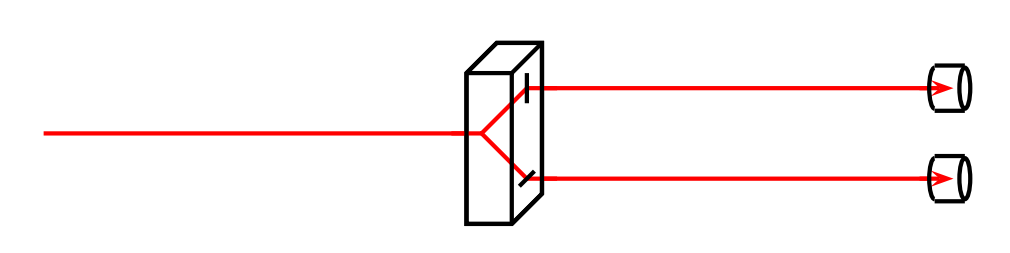
\includegraphics[scale=0.5]{img/dvolomac_detektor.png}
\caption{Dvolomac s dva detektora} 
\end{figure}

Nakon detekcije, foton je apsorbiran i ne može se više mjeriti. Takav kvantnomehanički sustav, koji je moguće samo jednom izmjeriti u samo jednom od dva moguća stanja nazivamo \textbf{kvantnim bitom} ili \textbf{qubitom}.
Kvantni bit prije mjerenja može biti u beskonačno mnogo različitih stanja te općenito jedno takvo stanje zovemo \textbf{superpozicijom} dvaju stanja. Ta dva stanja se odnose na stanja baze koja mogu biti proizvoljna, ali su uvijek međusobno ortogonalna. Pojam superpozicije se može primijeniti i u klasičnom smislu. U slučaju svjetlosti, uzimajući dva linearno polarizirana vala s okomitim smjerovima polarizacije kao bazu sustava, općenito stanje polarizacije vala možemo prikazati kao:
\begin{equation}
E = E_x \hat{x}e^{i(\omega t + \phi_x)} + E_y \hat{y}e^{i(\omega t + \phi_y)} = E_0(\lambda \hat{x} + \mu \hat{y})e^{i\omega t}
\end{equation}
gdje vrijedi:
\begin{equation}
E_0 = \sqrt{(E_x^2 + E_y^2)}
\qquad
\lambda = \frac{E_x}{E_0}e^{i\phi_x}
\qquad
\mu = \frac{E_y}{E_0}e^{i\phi_y}
\qquad
|\lambda|^2 + |\mu|^2 = 1
\end{equation}
Bitno je uočiti da su $\lambda$ i $\mu$ kompleksni brojevi kao i da dio izraza $\lambda\hat{x}+\mu\hat{y}$ sadrži informaciju o stanju polarizacije vala te da takvih stanja ima beskonačno mnogo.

\subsection{Diracova notacija}

% DIRACOVA NOTACIJA i sva pravila - Hilbertov prostor itd
% izracunati vjerojatnost
% vektorski prikaz

\subsection{Prikaz na klasičnom računalu}










\section{Sustav kvantnih bitova i spregnutost}

\section{Kvantni operatori}

\section{Kvantni paralelizam}

\section{Kvantni logički kurg}

\chapter{Kvantni algoritmi}

\section{Kvantni paralelizam}

Kvantni paralelizam je svojstvo kvantnih računala da izvrše neku operaciju nad više mogućih ulaza odjednom. To svojstvo proizlazi iz prirode kvantnih bitova koja im omogućava da se nalaze u superpoziciji stanja. Za višestruku evaluaciju neke funkcije $f$, klasično računalo mora evaluirati $f$ više puta za različite ulaze, no kvantno računalo može tu istu funkciju evaluirati samo jednom i dobiti vektor stanja koji je težinska superpozicija svih mogućih izlaza. Takvo svojstvo se možda na prvi pogled ne čini previše korisnim, ali postoje algoritmi i situacije gdje se takvo svojstvo pokazalo iznimno korisnim, ponajviše kada je bitno neko općenito svojstvo funkcije.

\begin{figure}[H]
\centering
\begin{quantikz}
\lstick{$\ket{0}$} & \gate{H} & \qw  \\
\lstick{$\ket{0}$} & \gate{H} & \qw \\
\ldots \\
\lstick{$\ket{0}$} & \gate{H} & \qw \\
\end{quantikz}
\caption{Postavljanje bitova u stanje superpozicije}
\end{figure}

Iz tog razloga, veliki broj kvantnih algoritama kao prvi korak ima postavljanje svih kvantnih bitova u stanje superpozicije korištenjem Hadamardovih operatora što se često označava operatorom $H^{\otimes N}$ gdje je $N$ broj kvantnih bitova.



\section{Prevrtanje faze}

Prevrtanje faze je pojava kada ciljni bit CU operatora utječe na upravljački bit mijenjajući mu fazu. Javlja se kada je ciljni bit postavljen u svojstveno stanje unarnog operatora i kada je upravljački bit u jedinici. U takvoj situaciji, upravljački bit će primiti fazu od ciljnog bita, tj. pomnožiti će se svojstvenom vrijednosti unarnog operatora koja odgovara svojstvenom stanju ciljnog bita. Pošto je unarni operator unitaran, njegove svojstvene vrijednosti će uvijek biti oblika $e^{i\phi}$ što utječe samo na fazu.

\begin{figure}[H]
\centering
\begin{quantikz}
\lstick{$\ket{x}$} & \ctrl{1} & \qw \\
\lstick{$\ket{+}$ ili $\ket{-}$} & \targ{} & \qw
\end{quantikz}
\caption{Prevrtanje faze}
\end{figure}
Na primjeru operatora CX, svojstvena stanja operatora X su $\ket{+}$ i $\ket{-}$ uz svojstvene vrijednosti $\pm 1$. Jednostavnim izračunom se dobije:
\[
CNOT\ket{0+} = \ket{0+} \qquad
CNOT\ket{0-} = \ket{0-} \]
\[
CNOT\ket{1+} = 1 \cdot \ket{1+} \qquad
CNOT\ket{1-}= -1\cdot \ket{1-}\]
\[
CNOT\ket{++} = \ket{++} \qquad
CNOT\ket{+-} = \ket{- -} \]
\[
CNOT\ket{-+} = \ket{-+} \qquad
CNOT\ket{--} = \ket{+-}
\]

Prevrtanje faze je svojstvo koje se često koristi u kvantnim algoritmima zbog kojeg se neki bitovi inicijaliziraju u $\ket{1}$ prije primjene Hadamardovog operatora.
\begin{figure}[H]
\centering
\begin{quantikz}
\lstick{$\ket{0}$} & \qw & \gate{H} & \qw  \\
\lstick{$\ket{0}$} & \qw & \gate{H} & \qw \\
\ldots \\
\lstick{$\ket{0}$} & \qw & \gate{H} & \qw \\
\lstick{$\ket{0}$} & \gate{X} &\gate{H} & \qw \\
\end{quantikz}
\caption{Česta inicijalizacija kvantnog logičkog kruga}
\end{figure}
No, u praksi stanje kvantnog sustava na početku kvantnog logičkog kruga uvijek bude inicijalizirano u $\ket{00\ldots 00}$, pa je potrebno samo primijeniti operator X na kvantni bit koji treba biti u jedinici.

\section{Deutschev algoritam}

\subsection{Opis}

Deutschev algoritam jedan je od najjednostavnijih primjera kvantnog paralelizma koji demonstrira kvantnu nadmoć nad klasičnim računalom. Problem koji Deutschev algoritam rješava jest određivanje je li neka funkcija crne kutije oblika $f : \{0, 1\} \rightarrow \{0, 1\}$ \emph{uravnotežena} ili \emph{konstantna}. Postoje četiri takve funkcije:
\[
f(x) = 0
\qquad
f(x) = 1
\qquad
f(x) = x
\qquad
f(x) = \lnot x
\]
gdje su prve dvije konstantne, a druge dvije uravnotežene. Za rješavanje ovog problema, klasično računalo treba evaluirati funkciju barem dva puta, dok na kvantnom računalu funkciju je dovoljno evaluirati samo jednom.

Kvantni logički krug Deutschevog algoritma prikazan je kao:
\begin{figure}[H]
\centering
\begin{quantikz}
\lstick{$\ket{0}$} & \qw\slice{$\ket{\Phi_0}$}
& \gate{H}\slice{$\ket{\Phi_1}$} & \gate[wires=2][2cm]{U_f}\gateinput{$x$} \gateoutput{$x$}\slice{$\ket{\Phi_2}$} & \gate{H}\slice{$\ket{\Phi_3}$} & \meter{} \\
\lstick{$\ket{0}$} & \gate{X} & \gate{H} & \gateinput{$y$}\gateoutput{$y\oplus f(x)$} & \qw & \qw
\end{quantikz}
\caption{Kvantni logički krug Deutschevog algoritma}
\end{figure}
$U_f$ je kvantna implementacija funkcije $f$ za koju vrijedi:
\[
U_f\ket{x\otimes y} = \ket{x\otimes (y \oplus f(x))}
\qquad
x, y \in \{0, 1\}
\]
Na kraju logičkog kruga, izmjerena vrijednost prvog kvantnog bita iznosi 0 za konstantne funkcije, a 1 za uravnotežene.

\subsection{Analiza toka algoritma}
Razlog takvom ishodu može se pronaći analizirajući tok algoritma. Prije primjene Hadamardovih vrata sustav se nalazi u stanju:
\[
\ket{\Phi_0} = \ket{0\otimes 1}
\]
Nakon Hadamardovih vrata:
\[
\ket{\Phi_1} = \ket{+-} = \frac{1}{\sqrt{2}}(\ket{0} + \ket{1})\otimes\ket{-}
= \frac{1}{\sqrt{2}}(\ket{0-} + \ket{1-})
\]
Primjenom $U_f$ na stanje $\ket{x-}$ gdje je $x = \{0, 1\}$ dobiva se:
\begin{align*}
U_f\ket{x-} &= \frac{1}{\sqrt{2}}(U_f\ket{x0} - U_f\ket{x1}) \\
&= \frac{1}{\sqrt{2}}(\ket{x}\otimes\ket{f(x)} - \ket{x}\otimes\ket{f(x)\oplus 1})
\end{align*}
Uvrštavanjem 0 i 1 umjesto $f(x)$ dobiva se:
\[
U_f\ket{x-} =
\begin{cases}
\frac{1}{\sqrt{2}}(\ket{x0} - \ket{x1}) = \ket{x-} & \text{za} f(x) = 0 \\
\frac{1}{\sqrt{2}}(\ket{x1} - \ket{x0}) = -\ket{x-} & \text{za} f(x) = 1
\end{cases}
\]
odnosno:
\[
U_f\ket{x-} = (-1)^{f(x)}\ket{x-}
\]
Sada, primjenom $U_f$ na stanje $\ket{\Phi_1}$ dobije se $\ket{\Phi_2}$:
\begin{align*}
\ket{\Phi_2} &= U_f\ket{\Phi_1} = \frac{1}{\sqrt{2}}(U_f\ket{0-}+U_f\ket{1-}) \\
&= \frac{1}{\sqrt{2}}((-1)^{f(0)}\ket{0-} + (-1)^{f(1)}\ket{1-}) \\
&= \frac{(-1)^{f(0)}\ket{0} + (-1)^{f(1)}\ket{1}}{\sqrt{2}}\otimes\ket{-}
\end{align*}
Očigledno je da su stanja separabilna, stoga se prvi bit može promatrati samostalno. Primjenom Hadamardovih vrata na prvi kvantni bit dobiva se konačno stanje:
\begin{align*}
\ket{\Phi_3} &= H\cdot \frac{(-1)^{f(0)}\ket{0} + (-1)^{f(1)}\ket{1}}{\sqrt{2}} \\
&= \frac{(-1)^{f(0)}+(-1)^{f(1)}}{2}\ket{0} + \frac{(-1)^{f(0)}-(-1)^{f(1)}}{2}\ket{1}
\end{align*}
Iz jednadžbe se vidi da za konstantne funkcije vrijedi,
\[
\ket{\Phi_3} = \pm\ket{0}
\]
a za uravnotežene
\[
\ket{\Phi_3} = \pm\ket{1}
\]
Pošto faza nema utjecaja ne rezultate mjerenja, za konstantne funkcije rezultat mjerenja uvijek bude 0, a za uravnotežene 1.

\subsection{Deutsch-Joszin algoritam}

Postoji generalizacija ovoga algoritma pod nazivom Deutsch-Jozsin algoritam koji rješava isti problem, ali sa ulazom proizvoljnog broja bitova. U njemu je također potrebno evaluirati funkciju samo jednom gdje će izlazni registar biti u nulama ako je funkcija konstantna, a bilo što drugo ako je uravnotežena. U njega ovaj rad neće ulaziti, ali je sličan i može se pogledati u \citep{nielsen2010quantum}

Deutschev i Deutsch-Joszin algoritam dobro demonstriraju situaciju gdje je kvantno računalo puno efikasnije od klasičnog, ali za sada ne postoje neke korisne primjene tih algoritama.

\section{Groverov algoritam}

\subsection{Opis}
Groverov algoritam\citep{grover} jedan je od algoritama koji je definirao principe kvantnih algoritama pretraživanja. U načelu, problem koji rješava jest pretraživanje nestrukturirane baze podataka. Klasično računalo taj problem rješava u prosječno $N/2$ koraka, dok kvantno računalo implementirajući Groverov algoritam pronađe rješenje s visokom vjerojatnošću u samo $\sqrt{N}$ koraka.

Definirati Groverov algoritam kao algoritam pretraživanja nestrukturirane baze podataka malo je zavaravajuće jer se u praktičnom smislu nikada ne bi mogao koristiti za točno to. Prikladnija primjena Groverovog algoritma bila bi pronalaženje inverza funkcije što čak i zvuči puno zanimljivijim i korisnijim. Jedna takva funkcija jest kriptografska funkcija sažetka. Groverov algoritam može pronaći kolizije takve funkcije u $\sqrt{N}$ koraka gdje je $N$ veličina domene funkcije, što klasično računalo u načelu može izračunati samo grubom silom\footnote{Groverov algoritam se na neki način može interpretirati kao algoritam grube sile kvantnog računala, ali je kao takav i dalje eksponencionalno brži od klasičnog}.

Kvantni logički krug Groverovog algoritma može se prikazati kao: 
\begin{figure}[H]
\centering
\begin{quantikz}
\lstick{$\ket{0^{\otimes n}}$} & 
\gate{H^{\otimes n}}\slice{$\ket{s}$} & \qw & \qw &
\gate{U_f}\gategroup[wires=1, steps=2,style={dashed}]{Groverov operator} & 
\gate{U_s} & 
\meter{}
\end{quantikz}
\caption{Kvantni logički krug Groverovog algoritma}
\end{figure}

Groverov operator potrebno je primijeniti $\sqrt{N}$ puta gdje je $N = 2^n$, a $n$ broj kvantnih bitova. Sastoji se od kvantnog proroka \engl{quantum oracle} $U_f$ i difuzera \engl{diffuser} $U_s$. Kvantni prorok je jedinična matrica koja na mjestu jednog ili više elemenata kojeg tražimo umjesto jedinice ima $-1$. Difuzer je operator koji provodi operaciju $2\ket{s}\bra{s} - I_{2^n}$. Uzastopnim primjenjivanjem ovih operatora, stanje sustava se približava ciljnom stanju $\ket{w}$ koje želimo pronaći. Mjerenjem sustava nakon $\sqrt{N}$ primjena Groverovog operatora dobiva se traženi element s dovoljno velikom vjerojatnošću.

\subsection{Analiza toka algoritma}

Algoritam započinje kao i mnogi drugi, postavljanjem svih bitova u stanje superpozicije primjenom Hadamardovih operatora čime dobivamo stanje $\ket{s}$. Neka se traženo stanje zove $\ket{w}$ koji može biti ciljno stanje ili superpozicija ciljnih stanja ako ih ima više. Neka se vektor stanja koji je okomit na stanje $\ket{w}$ zove $\ket{s'}$. Takvo stanje može se dobiti oduzimanjem stanja $\ket{w}$ od stanja $\ket{s}$ i normiranjem. Stanja $\ket{w}$, $\ket{s}$ i $\ket{s'}$ mogu se nacrtati u dvodimenzioalnom prostoru:

\begin{figure}[H]
\centering
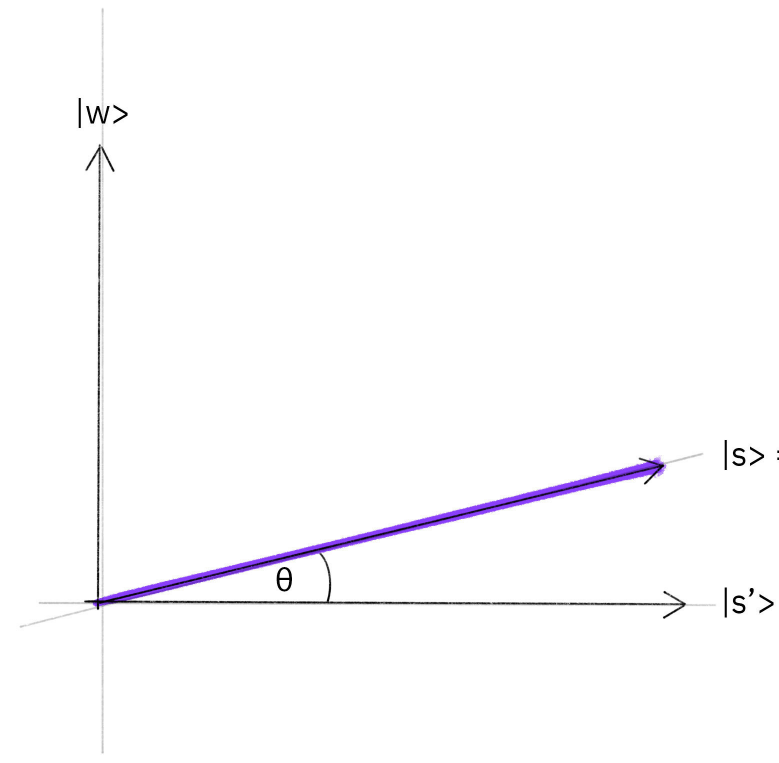
\includegraphics[scale=0.4]{img/grover1.png}
\end{figure}
gdje kut $\theta$ opisuje koliko je stanje $\ket{s}$ zakrenuto prema $\ket{w}$. Za njega vrijedi:
\[
\braket{s|w} = \frac{1}{\sqrt{N}} = \sin\theta \approx \theta
\]

Idući korak algoritma primjenjuje kvantni prorok $U_f$ na stanje $\ket{s}$. Sve što $U_f$ radi jest refleksiju oko stanja $\ket{s'}$:

\begin{figure}[H]
\centering
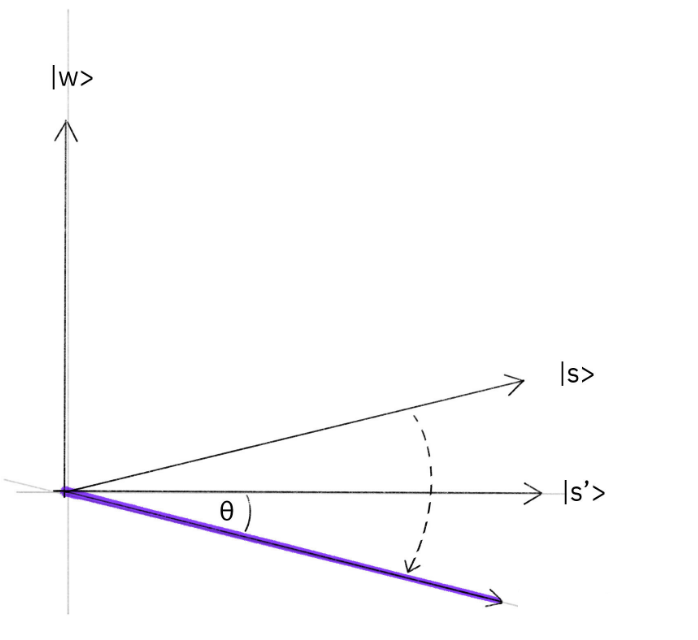
\includegraphics[scale=0.4]{img/grover2.png}
\end{figure}

Zatim se primjenjuje difuzer $U_s$ koji radi refleksiju oko stanja $\ket{s}$:

\begin{figure}[H]
\centering
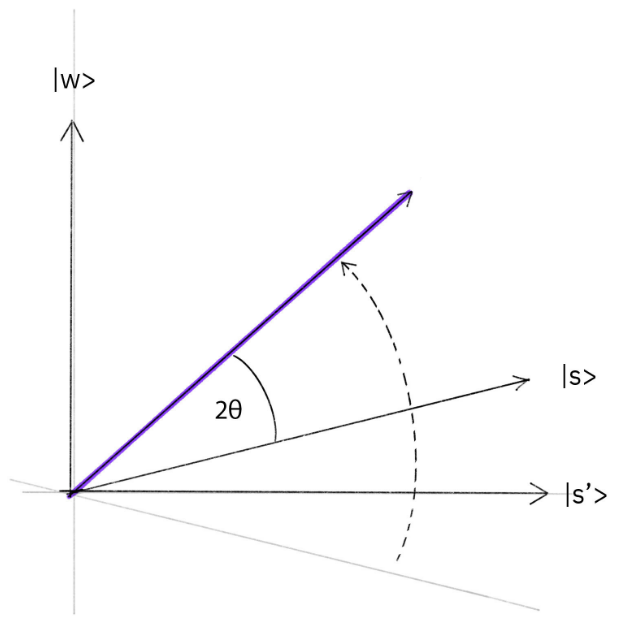
\includegraphics[scale=0.4]{img/grover3.png}
\end{figure}

Dakle, nakon jedne primjene Groverovog operatora, stanje $\ket{s}$ se zaokrenulo za dodatnih $2\theta$ prema ciljnom stanju $\ket{w}$. Nakon $k$ primjena Groverovog operatora, stanje $\ket{s}$ biti će za $(2k + 1)\theta$ zaokrenuto prema stanju $\ket{w}$. Cilj je da to bude što bliže stanju $\ket{w}$, dakle da vrijedi:
\[
(2k + 1)\theta \approx \frac{\pi}{2}
\]
Rješavajući jednadžbu za $k$, dobiva se:
\[
k \approx \frac{\pi}{4\theta} \approx \frac{\pi}{4}\sqrt{N} \approx \sqrt{N}
\]
što znači da je potrebno primijeniti Groverov operator približno $\sqrt{N}$ puta kako bi vjerojatnost mjerenja stanja $\ket{w}$ bila najveća.

\subsection{Kvantni prorok}

Neka je $U_f$ kvantni prorok Groverovog algoritma koji traži stanje $\ket{10}$. Njegova vrijednost iznosi:
\[
U_f = \begin{bmatrix}
1 & 0 & 0 & 0 \\
0 & 1 & 0 & 0 \\
0 & 0 & -1 & 0 \\
0 & 0 & 0 & 1
\end{bmatrix}
\]

Čini se kao da je za samu izgradnju logičkog kruga odnosno proroka potrebno poznavati rješenje koje tražimo što poništava cijeli smisao Groverovog algoritma. To je donekle i istina; poznavanjem matrične reprezentacije proroka, moguće je odrediti ciljna stanja, ili obratno, za konstrukciju proroka na ovakav način, potrebno je poznavati ciljna stanja. Iz toga slijedi da je Groverov algoritam koristan jedino kada se prorok tretira kao crna kutija ili ako se prorok konstruira na način gdje njegova vrijednost nije očita, ali da i dalje daje ispravan rezultat. Takva konstrukcija proroka postiže se koristeći prevrtanje faze.

Neka je $f$ kriptografska funkcija sažetka za koju vrijedi $f : \{0, 1\}^n \rightarrow \{0, 1\}^m$ te neka je njoj potrebno pronaći inverz.
\begin{figure}[H]
\centering
\begin{quantikz}
\lstick[wires=3]{$n = 3$} & \gate[wires=6][2cm]{U_{hash}} & \qw & \qw & \qw & \gate[wires=6][2cm]{U_{hash}^\dagger} & \qw \\
\qw & \qw & \qw & \qw & \qw & \qw &\qw \\
\qw & \qw & \qw & \qw & \qw & \qw & \qw \\
\lstick[wires=3]{$m = 3$} & & \qw & \ctrl{3} & \qw & \qw & \qw \\
\qw &  & \gate{X} & \ctrl{2} & \gate{X} & \qw & \qw \\
\qw & & \qw & \ctrl{1} & \qw & \qw & \qw \\
\lstick{$\ket{-}$} & \qw & \qw & \targ{} & \qw & \qw  & \qw
\end{quantikz}
\caption{Primjer kvantnog proroka za pronalaženje inverza od $\ket{101}$}
\end{figure}
Za implementaciju kvantnog proroka potrebno je $n + m + 1$ kvantnih bitova od kojih su $m + 1$ pomoćni. Prvih $n$ bitova se očekuje da su u stanju superpozicije, idućih $m$ bitova se postavlja u stanje $\ket{0}$, dok se zadnji bit postavlja u stanje $\ket{-}$. Zatim je potrebno u kvantnom logičkom krugu implementirati samu funkciju $f$ na način da joj je ulazni registar prvih $n$ bitova, a izlazni idućih $m$ bitova. Koristeći Toffolijeva vrata sa $m$ upravljačkih bitova, može se odabrati izlaz funkcije kojemu je potrebno pronaći inverz (na slici je to $f(x) = 101$). Ciljni bit Toffolijevih vrata je poslijednji bit koji je u stanju $\ket{-}$. Svrha Toffolijevih vrata je svakoj komponenti stanja koja rezultira željenim izlazom promijeniti predznak. To radi pomoću prevrtanja faze. Naime, vrijedi:
\[
CNOT\ket{0-} = \ket{0-} \qquad
CNOT\ket{1-} = -\ket{1-}
\]
Pošto se prorok koristi iterativno u algoritmu, potrebno je vratiti svih $m$ izlaznih kvantnih bitova u stanje nule. To se može postići primjenom operatora $f^\dagger$, koji često zna biti jednak $f$.

\section{Shorov algoritam}

\subsection{Opis problema}

Shorov algoritam rješava problem faktorizacije velikih brojeva. To je problem na čiju se tešku izračunljivost oslanja veliki dio modernih kriptografskih mehanizama. Dobar primjer toga jest RSA kriptosustav čija se tajnost privatnog ključa temelji na težini računanja Eulerove funkcije koja se može svesti na problem faktorizacije brojeva. Iz algoritma generiranja ključeva i funkcija enkripcije i dekripcije može se vidjeti zašto je to tako.

Algoritam generiranja ključeva:
\begin{enumerate}
\item Generiranje broja $N = p\cdot q$, gdje su $p$ i $q$ veliki slučajno odabrani prosti brojevi
\item Računanje Eulerove funkcije\footnote{Eulerova funkcija računa broj koji opisuje koliko relativno prostih faktora ima neki broj, tj. veličinu raduciranog sustava ostataka, no ovdje važnije svojstvo Eulerove funkcije jest da ako vrijedi $nzd(a, N) = 1$ onda isto vrijedi $a^{\varphi(N)} \equiv 1\mod N$ } $\varphi(N) = (p-1)(q-1)$
\item Odabir proizvoljnog broja $e$ iz reduciranog sustava ostataka modulo $\varphi(N)$
\item Računanje $d = e^{-1}$ u reduciranom sustavu ostataka modulo $\varphi(N)$
\item Javni ključ: pk = (e, N)
\item Privatni ključ: sk = (d, N)
\end{enumerate}

Funkcija enkripcije:
\[
E(m, (e,N)) = m^e \mod N
\]

Funkcija dekripcije:
\[
D(c,(d,N)) = c^d \mod N
\]

Ovo funkcionira jer vrijedi $e\cdot d = 1\mod \varphi(N)$, tj.
\[
D(m^e,(d,N)) = m^{e\cdot d} \mod N = m \mod N
\]

Dakle, kako bi se narušila sigurnost ovakvog sustava potrebno je moći efikasno izračunati proste faktore, odnosno $\varphi(N)$.

\subsection{Kvantna Fourierova transformacija}

Kvantna Fourierova transformacija vrši transformaciju baze računanja iz Z-baze (nazvane po osima Blochove sfere) u X-bazu koja se često zove Fourierovom bazom. Svaki broj koji se može prikazati stanjima $\ket{0}$ i $\ket{1}$ ima svoju reprezentaciju u Fourierovoj bazi zapisanu pomoću različitih rotacija oko osi Z. 

Broj 0 u Fourierovoj bazi ima sve kvantne bitove postavljene u $\ket{+}$. Za svaki idući broj, najniži bit se rotira oko osi Z za $\frac{1}{2^n}\cdot 2\pi$ radijana, drugi najniži za $\frac{2}{2^n}\cdot 2\pi$ radijana, treći za $\frac{4}{2^n}\cdot 2\pi$ radijana itd. Na primjer, broj 9 ($\ket{1001}$ u Z-bazi) u Fourierovoj bazi izgleda:
\begin{figure}[H]
\centering
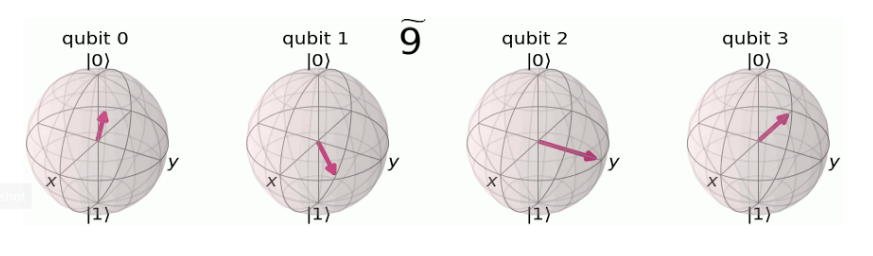
\includegraphics[scale=0.65]{img/Fourier9.png}
\caption{Broj 9 u Fourierovoj bazi s 4 kvantna bita}
\end{figure}

\begin{figure}[H]
\centering
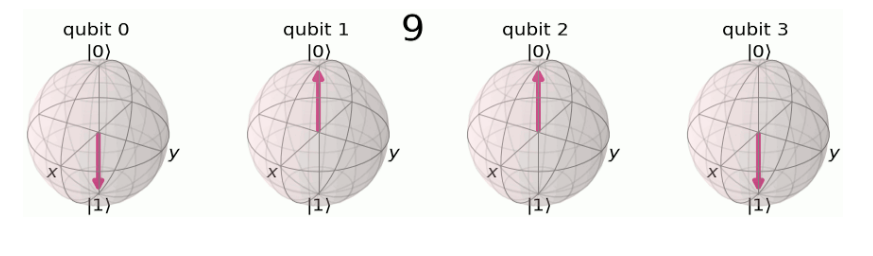
\includegraphics[scale=0.65]{img/Zbase9.png}
\caption{Broj 9 u Z-bazi s 4 kvantna bita}
\end{figure}

Vidi se da je najniži kvantni bit (qubit 0) zaokrenut oko osi Z za $\frac{9}{16}\cdot 2\pi$ radijana, drugi najniži (qubit 1) za $\frac{18}{16}\cdot 2\pi = \frac{2}{16}\cdot 2\pi$ radijana, treći za $\frac{36}{16}\cdot 2\pi = \frac{4}{16}\cdot 2\pi$ radijana i poslijednji za $\frac{72}{16}\cdot 2\pi = \frac{8}{16}\cdot 2\pi$ radijana.


U matematičkom smislu, kvantna Fourierova transformacija vrši transformaciju vektora stanja $\sum_{i=0}^{N-1}x_i\ket{i}$ u vektor stanja $\sum_{i=0}^{N-1}y_i\ket{i}$ gdje vrijedi:
\[
y_k = \frac{1}{\sqrt{N}}\sum_{j=0}^{N-1}x_j e^{\frac{2\pi i}{N}\cdot jk}
\]
Unitarna matrica kvantne Fourierove transformacije može se prikazati kao:
\[
U_{QFT} = \frac{1}{\sqrt{N}}\sum_{x=0}^{N-1}\sum_{y=0}^{N-1}\omega_N^{xy}\ket{y}\bra{x} 
= \frac{1}{\sqrt{N}}\begin{bmatrix}
1 & 1 & 1 & 1 & \dots & 1 \\
1 & \omega & \omega^2 & \omega^3 & \dots & \omega^{N-1} \\
1 & \omega^2 & \omega^4 & \omega^6 & \dots & \omega^{2(N-1)} \\
1 & \omega^3 & \omega^6 & \omega^9 & \dots & \omega^{3(N-1)} \\
\vdots & \vdots & \vdots & \vdots & \ddots & \vdots \\
1 & \omega^{N-1} & \omega^{2(N-1)} & \omega^{3(N-1)} & \dots & \omega^{(N-1)(N-1)} \\
\end{bmatrix}
\]
gdje je $\omega_N^{jk} = e^{\frac{2\pi i}{n}\cdot jk}$. Hadamardov operator je najmanji $U_{QFT}$.

Općenito, može se izračunati:
\begin{align*}
U_{QFT}\ket{x} &= \frac{1}{\sqrt{N}}\sum_{y=0}^{N-1}\omega_N^{xy}\ket{y} \\
&= \ldots =
\frac{1}{\sqrt{N}}(\ket{0}+e^{\frac{2\pi i}{2}x}\ket{1})\otimes
(\ket{0}+e^{\frac{2\pi i}{2^2}x}\ket{1})\otimes
\ldots \otimes
(\ket{0}+e^{\frac{2\pi i}{2^n}x}\ket{1})
\end{align*}

Zbog unitarnosti operatora $U_{QFT}$, za transformaciju iz Fourierove baze u Z-bazu, potrebno je samo primijeniti operator $U_{QFT}^{\dagger}$. 


Postoji točno određen način kako se konstruira kvantni logički krug kvantne Fourierove transformacije, ali u sklopu izgradnje simulatora, dovoljno je poznavati samo njezin matrični oblik.

\subsection{Kvantna procjena faze}

Kvantna procjena faze je algoritam sam za sebe, ali je samo dio Shorovog algoritma. Neka je $U$ unitarni operator sa svojstvenim vektorom $\ket{\Phi}$ i odgovarajućom svojstvenom vrijednosti $e^{2\pi i\theta}$.
\[
U\ket{\Phi} = e^{2\pi i\theta}\ket{\Phi}
\]
Algoritam procjene faze procjenjuje $\theta$ za dani $U$.
\begin{figure}[H]
\centering
\begin{quantikz}
\lstick[wires=4]{$\ket{0}^{\otimes t}$} & \gate{H} & \qw & \qw & \qw & \ \ldots \ & \ctrl{4} & \gate[wires=4]{QFT^{\dagger}} & \qw \\
& \vdots & & & & \ \ldots \ &\qw & \qw & \qw \\
& \gate{H} & \qw & \ctrl{2} & \qw & \ldots \ & \qw & & \qw \\
& \gate{H} & \ctrl{1} & \qw & \qw & \ \ldots \ & \qw & & \qw \\
\lstick{$\ket{\Phi}$} & \qw & \gate{U^{2^0}} & \gate{U^{2^1}} & \qw & \ \ldots \ & \gate{U^{2^{t-1}}} & \qw & \qw 
\end{quantikz}
\caption{Kvantni logički krug kvantne procjene faze}
\label{krug:faza}
\end{figure}

Princip algoritma je zapisati fazu operatora $U$ na prvih $t$ bitova u Fourierovoj bazi koja se onda transformira u Z-bazu korištenjem inverza kvantne Fourierove transformacije što omogućuje njeno mjerenje. To se postiže prevrtanjem faze, tj. korištenjem upravljačkih $U$ vrata i inicijalizacijom stanja $\ket{\Phi}$ u svojstveno stanje operatora $U$.

Pošto je zapis vrijednosti $a$ u Fourierovoj bazi takav da $k$-ti bit napravi $\frac{a\cdot 2^k}{2^t}$ rotacija oko osi Z, potrebno je primijeniti točno $t$ control-$U^{2^k}$ operacija gdje $k \in \{0, 1,\ldots t - 1\}$ kao što je prikazano na slici \ref{krug:faza}.
\[
U^{2^k}\ket{\Phi} = U^{2k-1}U\ket{\Phi} = U^{2k-1}e^{2\pi i\theta} = \ldots = e^{2\pi i 2^k\theta}\ket{\Phi}
\]
Nakon primjene svih $k$ control-$U$ operatora, stanje sustava jest:
\[
\ket{\Phi_2} = \frac{1}{\sqrt{2}}
(\ket{0}+e^{2\pi i\theta 2^0}\ket{1})\otimes
(\ket{0}+e^{2\pi i\theta 2^1}\ket{1})\otimes
\ldots \otimes
(\ket{0}+e^{2\pi i\theta 2^{t-1}}\ket{1}) \otimes
\ket{\Phi}
\]
koje odgovara procjeni $\theta$ u Fourierovoj bazi tenzorski pomnoženo s $\ket{\Phi}$. Nakon toga se primjenjuje $QFT^{\dagger}$ i izvršava se mjerenje.

Ovaj algoritam samo procjenjuje fazu jer će dobiveni rezultat $x$ označavati fazu $\frac{x}{2^t}$ što znači da će u pravilu procjena biti točnija što je $t$ veći, ali je, naravno, za neke faze moguće dobiti potpuno precizan rezultat.

\subsection{Opis algoritma}

Shorov algoritam se temelji na činjenici da ako je moguće efikasno pronaći period od
\[
f(x) = a^x \mod N
\]
onda je moguće efikasno faktorizirati $N$. Iz tog razloga Shorov algoritam procjenjuje period unitarnog operatora $U$ koji vrši operaciju:
\[
U\ket{y} = \ket{ay\mod N}
\]
Svaki svojstveni vektor operatora $U$ može se zapisati kao:
\[
\ket{\Phi_s} = \frac{1}{\sqrt{r}}\sum_{k=0}^{r-1}e^{-\frac{2\pi i s k}{r}}\ket{a^k\mod N}
\]
Primjenom operatora $U$ na jedno takvo svojstveno stanje dobije se:
\[
U\ket{\Phi_s} = e^{\frac{2\pi i s}{r}}\ket{\Phi_s}
\]
Koristeći algoritam procjene faze sa svojstvenim stanjem $\ket{\Phi_s}$ dobije se procjena faze $\frac{s}{r}$. No, konstrukcija svojstvenog stanja $\ket{\Phi_s}$ zahtjeva poznavanje $r$. Srećom, superpozicijom svih svojstvenih stanja $\ket{\Phi_s}$ dobiva se stanje $\ket{1}$.
\[
\frac{1}{\sqrt{r}}\sum_{s=1}^{r-1}\ket{\Phi_s} = \ket{1}
\]
Primjenjujući algoritam procjene faze sa svojstvenim stanjem $\ket{1}$, zapisana faza biti će superpozicija svih faza oblika $\frac{s}{r}$ te će se mjerenjem izmjeriti samo jedna od njih. Ovo je odlično svojstvo jer ono što je zapravo bitno jest $r$ za koji vrijedi:
\[
a^r \mod N = 1 \qquad
r \mid \varphi(N)
\]

Algoritam se sastoji od dijela gdje se operacije mogu izvoditi na klasičnom računalu, i kvantnog dijela koji je samo opisana kvantna procjena faze funkcije. Algoritam je kako slijedi:
\begin{enumerate}
\item Odabire se nasumičan broj $1 < a < N$
\item Provjerava se je li $a$ relativno prost s $N$, ako nije, pronađen je faktor, algoritam završava
\item Koristi se kvantna procjena faze unitarnog operatora za kojega vrijedi $U\ket{y} = \ket{ay\mod N}$
\item Dobivena faza $\frac{x}{2^t}$ se reducira (aproksimira) na $\frac{s}{r}$ gdje je $r < N$ i cijeli broj. Ako se odmah ne dobije $r$ za koji vrijedi $a^r \mod N = 1$, ovaj korak treba ponoviti nekoliko puta. Ako se i dalje ne dobije zadovoljavajući $r$, onda treba ponovno početi od koraka 1
\item Ako je $r$ neparan ili $a^{r/2} \equiv -1 (\mod N)$, povratak na korak 1
\item Inače, $nzd(a^{\frac{r}{2}} + 1, N)$ i $nzd(a^{\frac{r}{2}} - 1, N)$ su netrivijalni faktori od $N$
\end{enumerate}
Funkcija $nzd(a, b)$ označava najmanjeg zajedničkog djelitelja od $a$ i $b$.







































\chapter{Simulacija kvantnog računala}

\section{Postojeći simulatori kvantnog računala}

Danas postoje biblioteke i \emph{toolkits} za simulaciju kvantnih računala kao što su Qiskit, QuTiP, staq ili neki od brojnih drugih od kojih se veliki broj može pronaći na Quantiki web stranici \citep{simulatori}.  Mnogi alati nude razne funkcionalnosti kao što su analiza tijeka izvođenja logičkog kruga ili razne načine vizualizacije stanja sustava, ali isto tako znaju imati zbunjujuću dokumentaciju i neintuitivan način korištenja.

Qiskit, s druge strane, je dobro dokumentiran i uglavnom ima vrlo praktično sučelje. Čak dopušta programiranje i izvršavanje kvantnih logičkih krugova na pravim IBM-ovim kvantnim računalima za koje je često potrebno čekati u redu za korištenje. Također nudi razne vizualizacije kvantnog logičkog kruga i stanja sustava, a uz korištenje nekih drugih Python biblioteka kao što je matplotlib, moguće je dodatno vizualizirati rezultate izvođenja.

Samostalno izrađen simulator u sklopu ovoga rada ima sučelje slično Qiskitu, no napisan je u jeziku C++ te je dizajniran da što jednostavnije omogući demonstraciju nekih od prethodno opisanih pojava i algoritama u ovom radu.

\section{Izrada simulatora kvantnog računala}

\subsection{Jednostavan simulator kvantnog računala SQS}

\textbf{Simple Quantum Simulator} ili \textbf{SQS}  osmišljen je kao \emph{header-only} biblioteka u jeziku C++. Kao takav je neovisan o platformi uz kompromis duljeg vremena prevođenja. Za operacije s vektorima i matricama SQS koristi biblioteku Eigen \citep{eigen} koja se također sastoji od isključivo \emph{header} datoteka što dodatno produljuje vrijeme prevođenja, ali je ono i dalje prihvatljivo. Za korištenje biblioteke potrebno je u zaglavlje programa staviti \emph{include} datoteke \emph{sqs.h}.

\subsection{Struktura}

SQS se temelji na tri glavne komponente koje se koriste za konstrukciju kvantnih logičkih krugova. To su \textbf{QOperator}, \textbf{QComponent} i \textbf{QCircuit}.

\subsubsection{Razred QOperator}
Razred QOperator predstavlja kvantni operator nad jednim ili više kvantnih bitova. Enkapsulira matricu operatora i sadrži informaciju o tipu operatora koji pomaže objektu tipa QComponent integrirati ga u logički krug. Korisnik ne mora brinuti o tipu operatora. Za instanciranje QOperatora korisniku su na raspolaganju konstante i funkcije za konstruiranje često korištenih kvantnih operatora. Konstante su redom: \textit{Eye}, \textit{Hadamard}, \textit{PauliX}, \textit{PauliY}, \textit{PauliZ}, \textit{CX}, \textit{CY}, \textit{CZ}, \textit{Toffoli} i \textit{SWAP}. Od funkcija to su:
\lstset{language=c++, tabsize=4, style=mystyle}
\begin{lstlisting}
QOperator CU(size_t controls, QOperator unitary);
QOperator Phase(double phase);
QOperator QFT(unsigned int qubits);
QOperator QFTDagger(unsigned int qubits);
\end{lstlisting}
Funkcija \textit{CU} prima dva argumenta: koliko ima upravljačkih bitova te unitarni operator kojim upravljaju. \textit{Phase} prima fazu operatora, a \textit{QFT} i \textit{QFTDagger} primaju nad koliko kvantnih bitova djeluju. Sve navedene konstante i funkcije nalaze se u datoteci \emph{ops.hpp} biblioteke. Matrice konstanti se nalaze u datoteci \emph{eigenconsts.hpp}, ali su donekle sakrivene od korisnika koristeći namespace \emph{sqs::Private}.

Korisnik također može stvoriti vlastiti QOperator inicijalizirajući ga s Eigen matricom u konstruktoru ili koristeći linearnu kombinaciju postojećih i vlastitih QOperatora i Eigen matrica. QOperator ne brine o svojoj unitarnosti te tu odgovornost ostavlja korisniku.

\subsubsection{Razred QComponent}

QComponent je odgovoran za prvi korak integracije kvantnih operatora u kvantni logički krug. Funkcionira na način da se u njega dodavaju objekti tipa QOperator ili QComponent uz navedene indekse kvantnih bitova nad kojim djeluju.
\begin{lstlisting}
void add(QOperator qop, std::vector<unsigned int> qubitPos);
void add(QOperator qop, unsigned int qPos);
void add(QOperator qop, unsigned int qPos1, unsigned int qPos2);
void add(QOperator qop, unsigned int qPos1, unsigned int qPos2,
	unsigned int qPos3);
void add(QComponent qcomp);
\end{lstlisting}
Ukoliko se radi o operatoru s upravljačkim bitovima, potrebno je njih prve navesti, neovisno kojim redoslijedom.

QComponent nastoji što više operatora staviti u paralelu što smanjuje količinu matrica koje je kasnije potrebno izračunati u koracima simulacije. Od ostalih funkcionalnosti, QComponent nudi:
\begin{lstlisting}
void setIterations(unsigned int times);
std::vector<unsigned int> getQubitRange();
const MX& calculateMatrix();
\end{lstlisting}
\emph{setIterations} postavlja koliko puta se komponenta treba ponoviti u logičkom krugu što je korisno za neke algoritme poput Groverovog, \emph{getQubitRange} računa koje kvantne bitove komponenta koristi, a \emph{calculateMatrix} računa matrični prikaz komponente. Zadnje dvije funkcije koristi QCircuit kako bi uspješno simulirao logički krug. \emph{MX} i ostali nestandardni tipovi koji se koriste su definirani u datoteci \emph{eigenconsts.hpp} i predstavljaju samo kraći zapis tipova Eigen matrica.

\subsubsection{Razred QCircuit}

QCircuit predstavlja kvantni logički krug u kojeg se ugrađuju komponente koje nastoji što je više moguće paralelizirati. Pri stvaranju objekta tipa QCircuit, u konstruktoru je potrebno navesti broj kvantnih bitova. Funkcionalnosti koje QCircuit nudi su:
\begin{lstlisting}
void add(QComponent qcomp);
void add(QOperator qop, std::vector<unsigned int> qubitPos);
void add(QOperator qop, unsigned int qPos1);
void add(QOperator qop, unsigned int qPos1, unsigned int qPos2);
void add(QOperator qop, unsigned int qPos1, unsigned int qPos2,
	unsigned int qPos3);
void execute();
void resetQubits();
void clearCircuit();
VX getStateVector();
std:.vector<double> probabilityVector();
std::map<unsigned int, unsigned int> measure(unsigned int times,
	unsigned int bits);
std::map<unsigned int, unsigned int> measure(unsigned int times);
void measureAndDisplay(unsigned int times, unsigned int bits);
void measureAndDisplay(unsigned int times);


\end{lstlisting}
\emph{execute} pokreće simulaciju kvantnog logičkog kruga, odnosno računa sve potrebne matrice te ih množi vektorom stanja koji je na početku inicijaliziran u $\ket{0}$. \emph{resetQubits} postavlja vektor stanja u početno stanje. \emph{clearCircuit} uklanja sve komponente iz logičkog kruga. \emph{getStateVector} vraća trenutni vektor stanja logičkog kruga, dok \emph{probabilityVector} vraća vektor vjerojatnosti. \emph{measure} vrši mjerenje onoliko puta koliko je navedeno prvim argumentom nad svim bitovima ili nad prvih onoliko bitova koliko je navedeno u drugom argumentu te vraća rezultate mjerenja kao mapu. \emph{measureAndDisplay} radi isto što i \emph{measure}, samo što ne vraća mapu nego odmah prikazuje rezultate mjerenja na standardnom izlazu.

\subsection{Izazovi pri implementaciji}

U suštini, simulator se može svesti na računanje tenzorskog produkta i matrično množenje, no situacija ipak nije toliko jednostavna. Sve matrične reprezentacije kvantnih operatora koji djeluju na dva ili više kvantnih bitova pretpostavljaju točno određen raspored bitova. Na primjer CNOT i Toffolijeva vrata pretpostavljaju da su svi bitovi jedan uz drugog i da su upravljački bitovi iznad ciljnog. To je vrlo ograničavajuće te je bilo potrebno pronaći način konstrukcije operatora koji djeluje na proizvoljno raspoređenim bitovima.

Za CU operator sa jednim upravljačkim bitom i jednim ciljnim bitom, to je uvijek moguće postići jer se on može rastaviti na zbroj tenzorskih produkata. Na primjer, CNOT operatori:


\begin{figure}[H]
\centering
\begin{quantikz}
\qw & \ctrl{1} & \qw & & & \targ{} & \qw \\
\qw & \targ{} & \qw & & &  \ctrl{-1} & \qw \\
\end{quantikz}
\caption{$CNOT_{1, 2}$ i $CNOT_{2,1}$ operatori}
\end{figure}

mogu se prikazati kao:
\begin{equation}
CNOT_{1,2} = \ket{0}\bra{0}\otimes I_2 + \ket{1}\bra{1}\otimes \sigma_x \qquad
CNOT_{2,1} = I_2 \otimes\ket{0}\bra{0} +  \sigma_x \otimes\ket{1}\bra{1}
\end{equation}

Općenito, ako se između upravljačkog i ciljnog bita nalazi $n$ drugih operatora koji ne utječu na upravljački ili ciljni bit, zajednička matrica se može dobiti na način:
\begin{equation}
U = \ket{0}\bra{0}\otimes U_1 \otimes \ldots \otimes U_n \otimes I_2 + \ket{1}\bra{1}\otimes U_1 \otimes \ldots \otimes U_n \otimes \sigma_x
\end{equation}
ili
\begin{equation}
U = I_2 \otimes U_1 \otimes \ldots \otimes U_n \otimes \ket{0}\bra{0} +  \sigma_x \otimes U_1 \otimes \ldots \otimes U_n \otimes \ket{1}\bra{1}
\end{equation}
gdje $U_i$ mogu biti bilo koji unitarni operatori, a $I_2$ ako nema operatora.

Ovo naizgled rješava samo dio problema, ali je zapravo jedina stvar koja je potrebna za konstrukciju svih ostalih operatora koji djeluju na proizvoljno raspoređenim  bitovima.

Razlog tome je što se SWAP vrata mogu konstruirati od CNOT vrata. Vrijedi 
\begin{figure}[H]
\centering
\begin{quantikz}
\qw & \gate[swap]{} & \qw \\
\qw &  & \qw
\end{quantikz} =
\begin{quantikz}
\qw & \ctrl{1} & \targ{} & \ctrl{1} & \qw \\
\qw & \targ{} & \ctrl{-1} & \targ{} & \qw \\
\end{quantikz}
\caption{SWAP vrata prikazana pomoću CNOT vrata}
\end{figure}
Posljedica ove činjenice jest da je moguće zamijeniti bilo koja dva kvantna bita u logičkom krugu. Dakle, prije svake primjene višebitnog operatora, simulator napravi potrebne zamjene kako bi bitovi odgovarali ulazima operatora, bez da ikako mijenja matricu samog operatora. Takav način omogućuje korištenje logičkih vrata kao što su višeupravljačka Toffolijeva vrata:
\begin{figure}[H]
\centering
\begin{quantikz}
\qw & \ctrl{3} & \qw \\
\qw & \qw & \qw \\
\qw & \ctrl{1} & \qw \\
\qw & \targ{} & \qw \\
\qw & \ctrl{-1} & \qw
\end{quantikz}
\caption{Višeupravljačka Toffolijeva vrata}
\label{multitoffoli}
\end{figure}
Općenito matricu višeupravljačkog operatora je lagano konstruirati: svi elementi na dijagonali se postave u jedinicu, a u donji desni kut se postavi na matricu ciljnog operatora. Dakle, simulator bi vrata \ref{multitoffoli} konstruirao na način:
\begin{figure}[H]
\centering
\begin{quantikz}
\qw &\qw & \ctrl{3} & \qw & \qw \\
\qw & \swap{3} & \ctrl{2} & \swap{3} & \qw \\
\qw & \qw  & \ctrl{1} & \qw & \qw\\
\qw & \qw  & \targ{} & \qw & \qw \\
\qw & \targX{} & \qw & \targX{} & \qw
\end{quantikz}
\caption{Realizacija vrata sa slike \ref{multitoffoli} u simulatoru}
\end{figure}

\section{Primjeri simulacije kvantnih logičkih krugova}

\subsection{Superpozicija}

Radi lakšeg upoznavanja sa simulatorom, prvih par primjera će biti jednostavni. Simulator započinje svoj rad u stanju $\ket{0}$, stoga za postavljanje bitova u superpoziciju potrebno je primijeniti Hadamardov operator na sve bitove. Mjerenje sustava trebalo bi rezultirati približno jednakom raspodjelom svih vrijednosti. Logički krug koji treba simulirati:
\begin{figure}[H]
\centering
\begin{quantikz}
\lstick{$\ket{0}$} & \qw & \gate{H} & \qw & \meter{} \\
\lstick{$\ket{0}$} & \qw & \gate{H} & \qw & \meter{} \\
\lstick{$\ket{0}$} & \qw & \gate{H} & \qw & \meter{} \\
\lstick{$\ket{0}$} & \qw & \gate{H} & \qw & \meter{}
\end{quantikz}
\end{figure}

i njemu odgovarajući kod:
\begin{lstlisting}
#include "sqs/sqs.h"

using namespace sqs;

int main() {
	/* stvaranje kvantnog logickog kruga */
	QCircuit qc(4);

	/* dodavanje Hadamardovog operatora na sve bitove,
		moguce napraviti i u for petlji */
	qc.add(Hadamard, {0, 1, 2, 3});

	/* pokretanje simulatora i mjerenje stanja na kraju 1000 puta */
	qc.execute();
	qc.measureAndDisplay(1000);
	
	return 0;
}
\end{lstlisting}

Dobiveni ispis:
\begin{lstlisting}
	|0000>: 63
	|0001>: 56
	|0010>: 64
	|0011>: 62
	|0100>: 61
	|0101>: 68
	|0110>: 59
	|0111>: 68
	|1000>: 55
	|1001>: 72
	|1010>: 50
	|1011>: 82
	|1100>: 59
	|1101>: 63
	|1110>: 62
	|1111>: 56
\end{lstlisting}

\subsection{Spregnutost}

Spregnutost označava neseparabilno stanje kvantnih bitova te ga je iznenađujuće jednostavno dobiti; potrebna su samo dva operatora. Logički krug za dobivanje spregnutog sustava dva kvantna bita jest:
\begin{figure}[H]
\centering
\begin{quantikz}
\lstick{$\ket{0}$} & \qw & \gate{H} & \ctrl{1} & \meter{} \\
\lstick{$\ket{0}$} & \qw & \qw & \targ{} & \meter{}
\end{quantikz}
\end{figure}

\begin{lstlisting}
#include "sqs/sqs.h"

using namespace sqs;

int main() {

	QCircuit qc(2);

	/* dodavanje Hadamardovog operatora na qubit 0 */
	qc.add(Hadamard, 0);

	/* dodavanje CNOT operatora gdje je qubit 0 upravljacki,
		a 1 ciljni*/
	qc.add(CX, 0, 1);

	qc.execute();
	qc.measureAndDisplay(1000);
	
	return 0;
}
\end{lstlisting}
Dobiveni ispis:
\begin{lstlisting}
|00>: 498
|11>: 502
\end{lstlisting}

Za tri kvantna bita, primjer je sličan:
\begin{figure}[H]
\centering
\begin{quantikz}
\lstick{$\ket{0}$} & \gate{H} 	& \ctrl{1} 	& \qw 		& \meter{} \\
\lstick{$\ket{0}$} & \qw 			& \targ{} 	&  \ctrl{1}	& \meter{} \\
\lstick{$\ket{0}$} & \qw 			& \qw 		&  \targ{}	& \meter{}
\end{quantikz}
\end{figure}
uz odgovarajući kod
\begin{lstlisting}
	QCircuit qc(3);

	qc.add(Hadamard, 0);

	qc.add(CX, 0, 1);
	qc.add(CX, 1, 2);

	qc.execute();
	qc.measureAndDisplay(1000);
\end{lstlisting}
Dobiveni ispis:
\begin{lstlisting}
	|000>: 487
	|111>: 513
\end{lstlisting}
Idući primjeri izvornog koda uglavnom neće sadržavati elemente zaglavlja i funkcije main, nego samo relevantne dijelove.

\subsection{Deutschev algoritam}

Za Deutschev algoritam potrebno je implementirati funkciju oblika $f : \{0, 1\} \rightarrow \{0, 1\}$ te odrediti je li ona uravnotežena ili konstantna.

Za konstante funkcije, implementacija je takva da postaje jasno zašto se uvijek dobiva $\ket{0}$ kada se izmjeri prvi bit, odnosno prvih $n$ bitova u Deutsch-Josza generalizaciji algoritma. Za funkciju $f(x) = 0$ implementacija se sastoji od praznih žica, odnosno jediničnih matrica, dok $f(x) = 1$ ima $\sigma_x$ operator na izlaznom bitu. Očigledno je da izlazni bit uopće ne interagira sa ulazom što rezultira da ulaz na kraju evaluacije crne kutije ostaje nepromijenjen.
\begin{figure}[H]
\centering
\begin{minipage}{.5\textwidth}
\centering
\begin{quantikz}
\qw  & \qw & \qw \\
\qw & \qw & \qw
\end{quantikz}
\caption{$f(x) = 0$}
\end{minipage}%
\begin{minipage}{.5\textwidth}
\centering
\begin{quantikz}
\qw  & \qw & \qw \\
\qw & \gate{X} & \qw
\end{quantikz}
\caption{$f(x) = 1$}
\end{minipage}
\end{figure}

Implementacije uravnoteženih funkcija također nisu komplicirane:
\begin{figure}[H]
\centering
\begin{minipage}{.5\textwidth}
\centering
\begin{quantikz}
\qw & \ctrl{1} & \qw \\
\qw & \targ{} & \qw
\end{quantikz}
\caption{$f(x) = x$}
\end{minipage}%
\begin{minipage}{.5\textwidth}
\centering
\begin{quantikz}
\qw & \ctrl{1} & \qw & \qw \\
\qw & \targ{} & \gate{X} & \qw 
\end{quantikz}
\caption{$f(x) = \neg x$}
\end{minipage}
\end{figure}
Ovdje se vidi da će prevrtanje faze imati ključnu ulogu pošto je izlazni bit inicijaliziran u $\ket{-}$, a ulazni u $\ket{+}$. Primjenom CNOT operatora, izlazni bit će ulaznom bitu promijeniti fazu rezultirajući da će se ulazni bit pronaći u stanju $\ket{-}$ koje prolaskom kroz Hadamardov operator postaje stanjem $\ket{1}$.

Kvantni logički krug Deutschevog algoritma:
\begin{figure}[H]
\centering
\begin{quantikz}
\lstick{$\ket{0}$} & \qw & \gate{H} & \gate[wires=2][2cm]{U_f} \gateinput{$x$} \gateoutput{$x$} & \gate{H} & \meter{} \\
\lstick{$\ket{0}$} & \gate{X} & \gate{H} & \gateinput{$y$}\gateoutput{$y\oplus f(x)$} & \qw & \qw
\end{quantikz}
\end{figure}
gdje $U_f$ odgovara jednoj od spomenutih implementacija. Sve funkcije možemo testirati na način:
\begin{lstlisting}
#include "sqs/sqs.h"

using namespace sqs;

void Deutsch(int i) {
	QCircuit qc(2);

	qc.add(PauliX, 1);
	qc.add(Hadamard, 0, 1);

	switch(i) {
		case 0: // f(x) = 0
			break;
		case 1: // f(x) = 1
			qc.add(PauliX, 1);
			break;
		case 2: // f(x) = x
			qc.add(CX, 0, 1);
			break;
		case 3: // f(x) = ~x
			qc.add(CX, 0, 1);
			qc.add(PauliX, 1);
			break;
		default:
			return;
	}

	qc.add(Hadamard, 0);

	qc.execute();
	qc.measureAndDisplay(1000);
}

int main() {

	std::string funcs[] = {	"f(x) = 0", "f(x) = 1",
					"f(x) = x", "f(x) = ~x"};

	for(int i = 0; i < 4; ++i) {
		std::cout << funcs[i] << std::endl;
		Deutsch(i);
	}

	return 0;
}
\end{lstlisting}
Dobije se očekivani rezultat:
\begin{lstlisting}
	f(x) = 0
	|00>: 497
	|10>: 503
	f(x) = 1
	|00>: 487
	|10>: 513
	f(x) = x
	|01>: 508
	|11>: 492
	f(x) = ~x
	|01>: 482
	|11>: 518
\end{lstlisting}
Napomena: desni bit je rezultat algoritma; u skici kvantnog logičkog kruga, bit koji je najviši je u ispisu bit najmanje težine.

\subsection{Groverov algoritam}

Groverovim algoritmom moguće je rješavati SAT probleme. Problem koji je potrebno riješiti programira se unutar kvantnog proroka algoritma.

Neka je taj problem dan kao:
\begin{equation}
(A\lor\neg B)\land (B\lor C)\land (\neg A)
\end{equation}
Korisno je da se taj izraz negira dva puta kako bi se dobio oblik sa isključivo operatorima logičkog I. Na taj način prorok je moguće izgraditi pomoću Toffolijevih vrata.
\begin{equation}
\neg(\neg A \land B) \land\neg(\neg B \land C) \land \neg(A)
\end{equation}
Jedna ovakva klauzula može se prikazati kao:
\begin{figure}[H]
\centering
\begin{quantikz}
\lstick{$A$} &\gate{X} & \ctrl{3} & \gate{X} & \qw\\
\lstick{$B$} & \qw & \ctrl{2} & \qw & \qw\\
\lstick{$C$} & \qw & \qw & \qw & \qw \\
\lstick{$C_1$} & \qw & \targ{} & \qw & \ldots & \qw & \gate{X} & \qw \\
\end{quantikz}
\end{figure}
Dakle, za svaku klauzulu potrebno je imati jedan dodatni kvantni bit kao i još jedan koji će provjeravati jesu li sve klauzule zadovoljene. Ta provjera služi kako bi se pomoću prevrtanja faze negirala sva ona stanja koja su rezultirala rješenjem. Nakon provjere potrebno je vratiti sve dodatne kvantne bitove u početno stanje, odnosno treba ponoviti sve klauzule obrnutim redoslijedom. Cijeli kvantni logički krug izgleda ovako:
\begin{figure}[H]
\centering
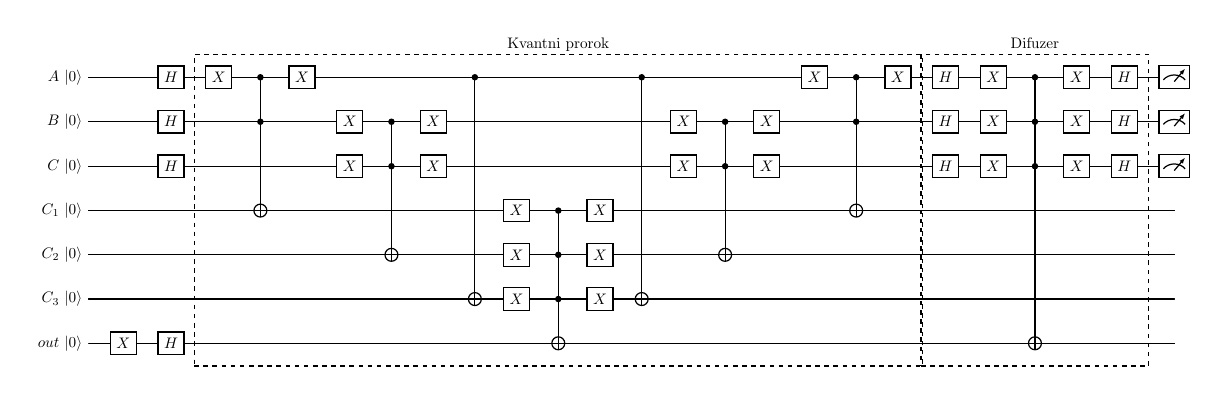
\begin{tikzpicture}
\node[scale=0.55]{
\begin{quantikz}
\lstick{$A$ $\ket{0}$} & \qw & \gate{H} & \gate{X}\gategroup[wires=7, steps=17,style={dashed}]{Kvantni prorok} & \ctrl{3} & \gate{X} & \qw & \qw & \qw & \ctrl{5} & \qw & \qw & \qw & \ctrl{5} & \qw & \qw & \qw & \gate{X} & \ctrl{3} & \gate{X} & \gate{H}\gategroup[wires=7, steps=5,style={dashed}]{Difuzer} & \gate{X} & \ctrl{6} & \gate{X} & \gate{H} & \meter{} \\
\lstick{$B$ $\ket{0}$} & \qw & \gate{H} &\qw & \ctrl{2} & \qw & \gate{X} & \ctrl{3} & \gate{X} & \qw & \qw & \qw & \qw & \qw & \gate{X} & \ctrl{3} & \gate{X} & \qw & \ctrl{2} &\qw & \gate{H} & \gate{X} & \ctrl{5} & \gate{X} & \gate{H} & \meter{}\\
\lstick{$C$ $\ket{0}$} & \qw & \gate{H} &\qw & \qw &\qw & \gate{X} & \ctrl{2} & \gate{X} & \qw & \qw & \qw & \qw & \qw & \gate{X} & \ctrl{2} &\gate{X} & \qw & \qw & \qw &\gate{H} & \gate{X} & \ctrl{4} & \gate{X} & \gate{H} & \meter{}\\
\lstick{$C_1$ $\ket{0}$} & \qw & \qw &\qw & \targ{} &\qw & \qw & \qw & \qw & \qw & \gate{X} & \ctrl{3} &\gate{X} & \qw & \qw & \qw &\qw & \qw & \targ{} & \qw & \qw & \qw &\qw & \qw & \qw & \qw \\
\lstick{$C_2$ $\ket{0}$} &\qw & \qw &\qw & \qw & \qw & \qw & \targ{} & \qw & \qw & \gate{X} & \ctrl{2}& \gate{X} &\qw & \qw & \targ{} &\qw & \qw & \qw & \qw & \qw & \qw & \qw & \qw & \qw & \qw \\
\lstick{$C_3$ $\ket{0}$} &\qw & \qw &\qw & \qw & \qw & \qw & \qw & \qw & \targ{} & \gate{X} & \ctrl{1}& \gate{X} & \targ{} & \qw & \qw & \qw & \qw & \qw & \qw & \qw & \qw & \qw & \qw & \qw & \qw \\
\lstick{$out$ $\ket{0}$} &\gate{X} & \gate{H} &\qw & \qw & \qw & \qw & \qw & \qw & \qw & \qw & \targ{} & \qw & \qw & \qw &\qw & \qw &\qw & \qw & \qw & \qw & \qw & \targ{} & \qw & \qw & \qw
\end{quantikz}
};
\end{tikzpicture}
\end{figure}

Difuzer neće biti objašnjen, ali kao što je prethodno spomenuto, on izvodi operaciju $2\ket{s}\bra{s} - I_{2^n}$ koja je zapravo samo refleksija vektora stanja oko uravnotežene superpozicije svih stanja $\ket{s}$.
Izvedba kvantnog logičkog kruga u simulatoru:
\begin{lstlisting}
	QCircuit qc(7);

	qc.add(PauliX, 6);
	qc.add(Hadamard, {0, 1, 2, 6});

	QComponent groverOperator;
	QComponent oracle;
	QComponent diffuser;

	/* A or ~B */
	oracle.add(PauliX, 0);
	oracle.add(Toffoli, 0, 1, 3);
	oracle.add(PauliX, 0);
	
	/* B or C*/
	oracle.add(PauliX, 1, 2);
	oracle.add(Toffoli, 1, 2, 4);
	oracle.add(PauliX, 1, 2);

	/* ~A */
	oracle.add(CX, 0, 5);

	oracle.add(PauliX, 3, 4, 5);
	oracle.add(CU(3, PauliX), {3, 4, 5, 6});
	oracle.add(PauliX, 3, 4, 5);

	/* obrnuti smjer */
	oracle.add(CX, 0, 5);
	oracle.add(PauliX, 1, 2);
	oracle.add(Toffoli, 1, 2, 4);
	oracle.add(PauliX, 1, 2);
	oracle.add(PauliX, 0);
	oracle.add(Toffoli, 0, 1, 3);
	oracle.add(PauliX, 0);
	

	/* difuzer */
	diffuser.add(Hadamard, 0, 1, 2);
	diffuser.add(PauliX, 0, 1, 2);
	diffuser.add(CU(3, PauliX), {0, 1, 2, 6});
	diffuser.add(PauliX, 0, 1, 2);
	diffuser.add(Hadamard, 0, 1, 2);
	
	groverOperator.add(oracle);
	groverOperator.add(diffuser);

	qc.add(groverOperator);
	qc.execute();
	qc.measureAndDisplay(1000, 3);
\end{lstlisting}

Groverov operator se u ovom primjeru primijenio samo jednom te je dobiveni rezultat:
\begin{lstlisting}
	|000>: 71
	|001>: 81
	|010>: 73
	|011>: 68
	|100>: 486
	|101>: 68
	|110>: 74
	|111>: 79
\end{lstlisting}
Vidi se da rezultat $\ket{100}$ ima najveću vjerojatnost mjerenja, te odgovara rješenju
\begin{equation}
A = False \qquad B = False \qquad C = True
\end{equation}
Komponentu groverOperator moguće je primijeniti više puta pozivom funkcije \emph{QComponent::setIterations(unsigned int times)} te bi se tada dobila veća vjerojatnost mjerenja točnog rezultata.

\subsection{Kvantna estimacija faze}

Ključan dio Shorovog algoritma je algoritam kvantne estimacije faze. U ovom konkretnom primjeru, estimirati će se faza samog operatora faze $P$. Operator faze ima oblik:
\begin{equation}
P[\varphi] = 
\begin{bmatrix}
1 & 0 \\ 0 & e^{i\varphi}
\end{bmatrix}
\end{equation}
stoga će kvantna estimacija faze izračunati $\frac{\varphi}{2}$. Za primjer, uzeti će se $\varphi = \frac{1}{2}$. Kvantni logički krug:
\begin{figure}[H]
\centering
\begin{quantikz}
\lstick{$\ket{0}$} & \gate{H} & \qw & \qw & \qw & \ctrl{3} & \ctrl{3} & \ctrl{3} & \ctrl{3} & \gate[wires=3]{QFT^{\dagger}} & \meter{} \\
\lstick{$\ket{0}$} & \gate{H} & \qw & \ctrl{2} & \ctrl{2} & \qw & \qw & \qw & \qw & \qw & \meter{}\\
\lstick{$\ket{0}$} & \gate{H} & \ctrl{1} & \qw & \qw &\qw & \qw & \qw & \qw & \qw & \meter{} \\
\lstick{$\ket{0}$} & \gate{X} & \gate{P(\frac{1}{2}} & \gate{P(\frac{1}{2}} & \gate{P(\frac{1}{2})} & \gate{P(\frac{1}{2})} & \gate{P(\frac{1}{2})} & \gate{P(\frac{1}{2})} & \gate{P(\frac{1}{2})} & \qw & \qw
\end{quantikz}
\end{figure}
Odgovarajući kod:
\begin{lstlisting}
	QCircuit qc(4);
	qc.add(PauliX, 3);
	qc.add(Hadamard, {0, 1, 2});

	QOperator ph = Phase(1.0 / 2.0); /* pi/2 = 2pi * (1/4) */
	QOperator cPh = CU(1, ph);

	qc.add(cPh, 0, 3);
	qc.add(cPh, 0, 3);
	qc.add(cPh, 0, 3);
	qc.add(cPh, 0, 3);
	qc.add(cPh, 1, 3);
	qc.add(cPh, 1, 3);
	qc.add(cPh, 2, 3);

	qc.add(QFTDagger(3), {0, 1, 2});
	qc.execute();

	auto m = qc.measure(1000, 3);
	for(auto a : m) {
		std::cout << a.first << "/8"
			<< "\tp: " << a.second / 10.0 << "%\n";  
	}
\end{lstlisting}
Dobiveni rezultat:
\begin{lstlisting}
	2/8     p: 100%
\end{lstlisting}
odgovara očekivanjima, naime $\frac{2}{8} = \frac{1}{4} = \frac{1/2}{2} = \frac{\varphi}{2}$.
\section{Prednosti i mane simulatora kvantnog računala}

Bilo koji simulator kvantnog računala nikada neće moći nadomjestiti pravo kvantno računalo što je posljedica same njegove prirode. Sustav od $n$ kvantnih bitova klasično računalo prikazuje vektorom dimenzije $2^n$, a svaki operator koji djeluje na taj vektor matricom dimenzije $2^n \times 2^n$. Uz problem pohrane takvih podataka za veliki broj kvantnih bitova, još je veći problem vrijeme izvršavanja operacija koje uključuju takve operande. Postoji fizička granica kada klasična računala više ne mogu u razumnom vremenu računati što se odvija u nekom kvantnom sustavu\footnote{Pojam kvantna nadmoć \engl{quantum supremacy} se odnosi točno na ovu granicu.}.

No, simulatori su daleko od toga da su beskorisni. Sama činjenica što su simulatori, a ne kvantni sustavi može pomoći pri analizi određenih svojstava kvantnih sustava. Simulator je u svakom trenutku moguće zaustaviti i analizirati stanje sustava bez da se naruši to stanje. Postoje neka ograničenja kvantnih računala koja ne postoji na klasičnim, kao što je na primjer nemogućnost kloniranja kvantnog bita ili nemogućnost višestrukog mjerenja sustava. Također je bitno spomenuti da u simulatorima ne postoji\footnote{Osim ako to namjerno nije simulirano} pojava dekoherencije koja smanjuje preciznost računanja u pravim kvantnim računalima.

U svakom slučaju, simulatori su odlični alati za eksperimentiranje, analizu i bolje shvaćanje kvantnih sustava, pogotovo ako pravo kvantno računalo nije lako dostupno.











\chapter{Zaključak}

\bibliography{literatura}
\bibliographystyle{fer}

\begin{sazetak}
Kvantna računala uvode novi način računanja koji znatno proširuje mogućnosti klasičnih računala i kao takva sadrže veliki potencijal koji se tek nedavno počeo ostvarivati. Ovaj rad se bavi osnovnim principima rada kvantnog računala kao i nekim bitnim konceptima koji se javljaju u kvantni logičkim krugovima kao što su spregnutost, kvantni paralelizam i prevrtanje faze. Nadalje, rad opisuje Deutschev, Groverov i Shorov algoritam te na kraju na samostalno izgrađenom simulatoru demonstrira neke od spomenutih pojava i algoritama.

\kljucnerijeci{simulator kvantnog računala, kvantno računalo, simulator, kvantni bit, qubit, kvantni algoritam. kvantni paralelizam, prevrtanje faze}
\end{sazetak}

% TODO: Navedite naslov na engleskom jeziku.
\engtitle{Quantum computer simulation}
\begin{abstract}
Quantum computers introduce a new way of computing that significantly expands the capabilities of classical computers and as such contain great potential that has only recently begun to be realized. This paper deals with the basic principles of quantum computing as well as some of the important concepts that occur in quantum logic circuits such as quantum entanglement, quantum parallelism, and phase kickback. Furthermore, the paper describes famous algorithms devised by D. Deutsch, L. K. Grover and P. W. Shor and finally demonstrates some of the mentioned phenomena and algorithms on a self-built simulator.

\keywords{quantum computer simulator, quantum computer, simulator, quantum bit, qubit, quantum algorithm, quantum parallelism, phase kickback}
\end{abstract}

\end{document}
